\newpage
\section{63. 不同路径 II}
\label{leetcode:63}

\subsection{题目}

一个机器人位于一个 m x n 网格的左上角 (起始点在下图中标记为``Start'')。

机器人每次只能向下或者向右移动一步。机器人试图达到网格的右下角(在下图中标记为``Finish'')。

现在考虑网格中有障碍物。那么从左上角到右下角将会有多少条不同的路径?

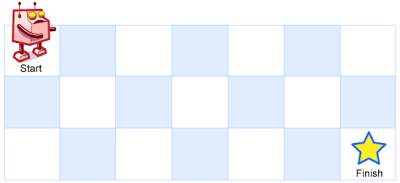
\includegraphics[width=120mm,height=60mm]{images/leetcode/robot_maze.png}

网格中的障碍物和空位置分别用 1 和 0 来表示。

\textbf{说明}:m 和 n 的值均不超过 100。

\textbf{示例 1}:

\begin{verbatim}
  输入:
  [
    [0,0,0],
    [0,1,0],
    [0,0,0]
  ]
  输出: 2
  解释:
  3x3 网格的正中间有一个障碍物。
  从左上角到右下角一共有 2 条不同的路径:
  1. 向右 -> 向右 -> 向下 -> 向下
  2. 向下 -> 向下 -> 向右 -> 向右
\end{verbatim}

\subsection{参考题解}

\paragraph{Python 代码}

\begin{verbatim}
class Solution:
  def uniquePathsWithObstacles(self, obstacleGrid: List[List[int]]) -> int:
    rows = len(obstacleGrid)
    cols = len(obstacleGrid[0])
    dp = [[0 for _ in range(cols)] for _ in range(rows)]

    if obstacleGrid[rows-1][cols-1] == 0:
      dp[rows-1][cols-1] = 1

    for row in range(rows-2, -1, -1):
      if obstacleGrid[row][cols-1] == 0 and dp[row+1][cols-1] == 1:
        dp[row][cols-1] = 1

    for col in range(cols-2, -1, -1):
      if obstacleGrid[rows-1][col] == 0 and dp[rows-1][col+1] == 1:
        dp[rows-1][col] = 1

    for row in range(rows-2, -1, -1):
      for col in range(cols-2, -1, -1):
        if obstacleGrid[row][col] == 1:
          dp[row][col] = 0
        else:
          dp[row][col] = dp[row+1][col] + dp[row][col+1]

    return dp[0][0]
\end{verbatim}
